\subsection{Regresión lineal}
La \textbf{Regresión Lineal}\index{Regresión!Lineal} es un potente algoritmo de \textit{machine learning} que 
permite predecir el comportamiento de una variable dependiente $y \in \mathds{R}$ a partir de los 
valores de la variable independiente $x \in \mathds{R}^n$.
El modelo se puede expresar como una ecuación o recta de regresión 
$$h_{\theta}(x) = \theta^T x = \theta_0 + \theta_1 x_1 + \cdots + \theta_n x_n$$
de la cual se debe ajustar el parámetro desconocido $\theta \in \mathds{R}^n$ para que el error 
de las predicciones sea el menor posible.

Dicho error viene representado por la función de perdida cuadrática
$$J(\theta) = \frac{1}{2m} \sum_{i=1}^{m}(\theta^Tx^{(i)} - y^{(i)})^2$$
donde $\theta^Tx^{(i)}$ representa el valor predecido para el ejemplo $i$-ésimo del \textit{dataset}, y la variable 
$y^{(i)}$ representa el valor real del ejemplo $i$-ésimo.

Gráficamente, en $\mathds{R}^2$, el problema consiste en ajustar lo mejor posible una recta a los 
puntos que representan los ejemplos de entrenamiento

\begin{figure}[h]
  \centering
  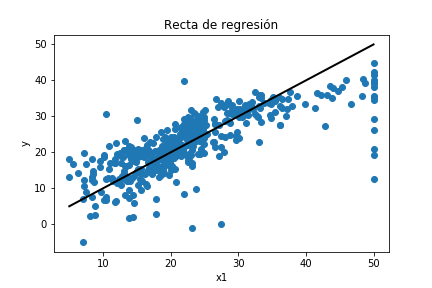
\includegraphics[width=\textwidth]{C:/Users/David/Desktop/TFG/TFGLatex/imagenes/recta_regresion.png}
  \caption[Regresión lineal en $\mathds{R}^2$]{Recta de regresión}
  \label{recta_regresion}
\end{figure}

\noindent \textbf{Gradiente de descenso}\\
Uno de los algoritmos mas populares de optimización de funciones es el algoritmo del Gradiente 
de Descenso\index{Gradiente de descenso} 
(\href{https://en.wikipedia.org/wiki/Gradient_descent}{\textit{Gradient Descent}}).
Este algoritmo consiste en actualizar los pesos o variables $\theta_i \enskip \forall i=1, \cdots, n$ de 
manera que con cada iteración se vaya reduciendo el error $J(\theta)$.
Las actualizaciones en cada iteración están dadas por la siguiente fórmula~\cite{DBLP:books/lib/Bishop07}

\begin{equation}
\theta := \theta - \alpha \frac{1}{m} \sum_{i=1}^{m}(h_{\theta}(x^{(i)}) - y^{(i)})x^{(i)}
\end{equation}

donde $\alpha$ es un parámetro que controla el salto que se produce en cada iteración del algoritmo, 
también denominado tasa de aprendizaje o \textit{learning rate}.
A valores pequeños del parámetro la iteración se vuelve mas lenta pero mas segura, por el contrario, 
valores grandes del parámetro producen que el algoritmo se acelere de manera considerable pero a costa 
de correr el riesgo de que incluso no llegue a converger.

\clearpage

Una manera lógica de paralelizar este computo es dividir el trabajo en el conjunto de entrenamiento 
de tal manera que cada máquina trabaje sobre un cierto numero de ejemplos de entrenamiento y no 
sobre el conjunto total.
Supongamos que nuestro conjunto de entrenamiento $X$ tiene un total de $m=4 \cdot 10^8$ de ejemplos.
Una iteración del algoritmo de descenso de gradiente tiene que recorrer todos los ejemplos y realizar 
un calculo con cada uno de ellos, sin embargo, definamos lo siguiente:
$$ temp^{(1)} = \sum_{i=1}^{10^8}(h_{\theta}(x^{(i)}) - y^{(i)})x^{(i)} $$
Este calculo sería realizado en una máquina (notese que solo utiliza un cuarto del \textit{dataset} original) 
de tal manera que esta máquina en particular solo contendría un cuarto del calculo total a realizar.
De manera análoga definimos
$$ temp^{(2)} = \sum_{i=10^8+1}^{2 \cdot 10^8}(h_{\theta}(x^{(i)}) - y^{(i)})x^{(i)} $$
que sería el calculo a realizar por la segunda máquina.
Así sucesivamente, hemos dividido el trabajo en 4 porciones que se desarrollan de manera totalmente 
independiente y paralela.\\
Sin embargo, el calculo de una iteración del gradiente de descenso no 
acaba aquí, ya que necesitamos combinar los resultados de estas cuatro máquinas.\\
Esto de nuevo en sencillo, ya que un ultimo cálculo requeriría juntar las cuatro porciones de la 
siguiente manera:
$$ \theta := \theta - \alpha \frac{1}{4 \cdot 10^8}(temp^{(1)} + temp^{(2)} + temp^{(3)} + temp^{(4)}) $$
De manera gráfica, para una paralelización en $n$ partes, cada partición de los datos se alojaría en un nodo
como un bloque de datos el cual sería procesado y luego enviado a través de la red a un nodo que recibiría
todas las partes y haría la agregación o combinación de los resultados.

\begin{figure}[h]
  \centering
  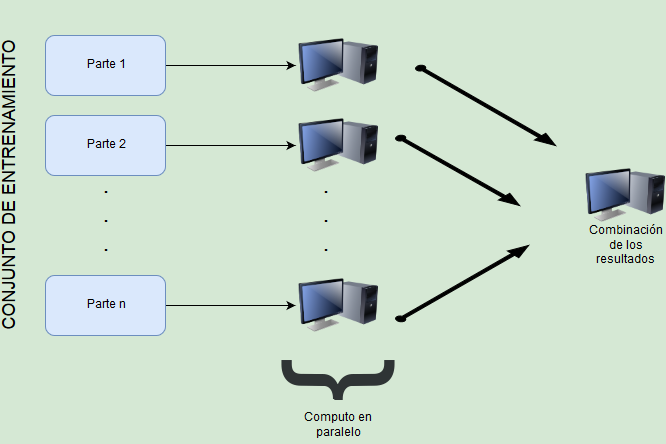
\includegraphics[width=\textwidth]{C:/Users/David/Desktop/TFG/TFGLatex/imagenes/computo_paralelo.png}
  \caption[División de los datos en el gradiente de descenso]
          {Computo en paralelo y agregación de los datos}
  \label{computo_paralelo}
\end{figure}

\newpage

\subsubsection*{Código \textit{Spark} Regresión lineal}
\lstinputlisting[caption=LinearRegression.py, language=Python, firstline=8]
                {C:/Users/David/Desktop/TFG/implementaciones/LinearRegression.py}

\begin{lstlisting}[language=bash, numbers=none]
$ spark-submit --master yarn-client LinearRegression.py
\end{lstlisting}

\clearpage

%TODO graficas del rendimiento del algoritmo


\subsection{Naive-Bayes}
Un clasificador \textbf{NaiveBayes}\index{NaiveBayes} es un clasificador probabilístico que se apoya en el 
\textit{Teorema de Bayes} para clasificar las entradas.
Es un modelo que asume que las características de las variables de entrada son independientes 
entre si, esto es, el valor de una cierta variable no influye para nada en el valor de otra.\\
La idea general detrás del algoritmo es calcular la media y la varianza de cada clase y cada característica.
Una vez realizado esto, se pueden utilizar los valores obtenidos para predecir la clase de un nuevo 
dato de entrada. El modelo lo etiquetará con la clase que mas se parezca de las vistas en el 
conjunto de entrenamiento.
\newline

Como se ha mencionado anteriormente, el algoritmo utiliza el teorema de Bayes para asignar la probabilidad de
un suceso condicionado a la ocurrencia de otro. En el ejemplo explicado mas abajo dichos sucesos serían la
probabilidad a priori y a posteriori de ser hombre o mujer.
%\newline

\begin{theorem}[Teorema de Bayes]\index{Teorema de Bayes}
  Sean ${A_1, A_2, \cdots, A_n}$ sucesos con $P(A_i) \neq 0 \quad \forall i=1, 2, \cdots, n$. 
  Sea $B$ un suceso cualquiera del que se conocen $P(B|A_i) \quad \forall i=1, 2, \cdots, n$.
  Entonces:
  {\fboxsep 8pt\fboxrule 1pt
  \begin{equation*}
  \fbox{$ P(A_i|B) = \frac{P(B|A_i) \cdot P(A_i)}{P(B)} $}
  \end{equation*}
  }
%  $$ P(A_i|B) = \frac{P(B|A_i) \cdot P(A_i)}{P(B) $$
\end{theorem}

Supongamos que queremos clasificar a una persona en hombre o mujer a través de características como 
la altura, el peso y el numero de pie. Aquí nuestras características serian $n=3$ y el objetivo 
sería predecir la variable $y=0$ si es hombre o $y=1$ si es mujer.
A partir de un \textit{dataset} de ejemplos etiquetados con hombre o mujer,
el concepto de aprendizaje para el algoritmo  sería calcular la media y la varianza 
de la altura, el peso y la talla de pie de todos los hombres y mujeres por separado.
Con estos datos, estamos en disposición de calcular la probabilidad a posteriori y las probabilidades 
condicionadas que servirán al algoritmo para realizar sus predicciones.

\begin{figure}[!htpb]
  \centering
  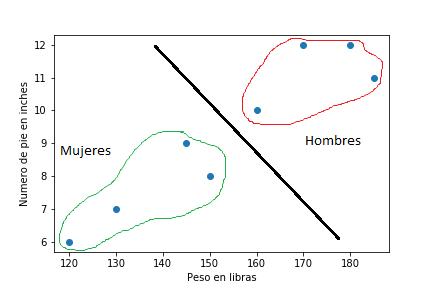
\includegraphics[width=\textwidth]{C:/Users/David/Desktop/TFG/TFGLatex/imagenes/naiveBayes_men_women.png}
  \caption[Naive Bayes clasificación]{Clasificación entre hombres y mujeres}
  \label{men_women_boundary}
\end{figure}

Debido a la simplicidad de los cálculos que usa para entrenarse, \textit{NaiveBayes} se desempeña muy bien 
en conjuntos de datos muy grandes dando lugar a modelos muy precisos.\\
Sin embargo, como todo modelo, tiene sus ventajas e inconvenientes que hacen de \textit{NaiveBayes} un modelo 
propicio para unos determinados tipos de problemas.

\clearpage

\begin{itemize}
  \item Ventajas:
  \begin{enumerate}
    \item Funciona muy bien en problemas multiclase. Dado un dato, es rápido y fácil predecir su clase.
    \item Asumiendo la independencia de las clases, un clasificador \textit{NaiveBayes} obtiene un mejor 
    desempeño comparado con otros métodos como la regresión logística, además necesita menos datos 
    de entrenamiento.
  \end{enumerate}
  \item Inconvenientes:
  \begin{enumerate}
    \item Si en los datos de test hay una característica nunca antes vista en los datos de 
    entrenamiento, el modelo le asignará una probabilidad de 0 y será incapaz de hacer una predicción.
    Esto es conocido como frecuencia cero o \textit{zero frequency}.
    \item En la vida real, es casi imposible encontrar un \textit{dataset} donde todas las características 
    sean completamente independientes unas de las otras.
  \end{enumerate}
\end{itemize}

\subsubsection*{Código MapReduce NaiveBayes}
\lstinputlisting[caption=NaiveBayes.py, language=Python, firstline=10]
                {C:/Users/David/Desktop/TFG/implementaciones/NaiveBayes.py}
                  
\begin{lstlisting}[language=bash, numbers=none]
$ python NaiveBayes.py <input_file> [-r hadoop]
\end{lstlisting}                
                    
\clearpage

%TODO graficas del rendimiento del algoritmo